%===============================================
%   rhnotes.tex — Framework for RH-coding Notes
%===============================================
\documentclass[11pt,a4paper]{article}

%----- ENHANCED TYPOGRAPHY -----
\usepackage[utf8]{inputenc}
\usepackage[T1]{fontenc}
\usepackage{lmodern}        % clean vector font
\usepackage{microtype}      % better justification & kerning
\usepackage[scaled=0.95]{helvet}  % sans serif for headings (optional)
\usepackage{mathpazo}       % Palatino for text & math

%----- PAGE LAYOUT -----
\usepackage{geometry}
  \geometry{top=1in, bottom=1in, left=1in, right=1in}
\usepackage{setspace}
  \onehalfspacing  % 1.5 line spacing

%----- FANCY HEADERS & FOOTERS -----
\usepackage{fancyhdr}
\pagestyle{fancy}
\fancyhf{}
% page number outside, header text inside
\fancyhead[LE]{\small Georges Khater}
\fancyhead[RE]{\small Notes on RH-coding}
\fancyhead[LO]{\small \rightmark}
\fancyhead[RO]{\small \leftmark}
\renewcommand{\headrulewidth}{0.4pt}
\renewcommand{\footrulewidth}{0pt}

% make sections feed into \leftmark/\rightmark
\renewcommand{\sectionmark}[1]{\markboth{#1}{}}
\renewcommand{\subsectionmark}[1]{\markright{#1}}

%----- SECTION NUMBERING & TOC DEPTH -----
\setcounter{secnumdepth}{3}  % number down to \subsubsection
\setcounter{tocdepth}{2}     % show ToC down to \subsection

%----- AMS MATH & THEOREM STYLES -----
\usepackage{amsmath,amssymb,mathtools}
\usepackage{amsthm}

% definitions, examples, remarks upright
\theoremstyle{definition}
\newtheorem{definition}{Definition}[section]
\newtheorem{example}[definition]{Example}
\newtheorem{remark}[definition]{Remark}

% theorems, lemmas, corollaries italic
\theoremstyle{plain}
\newtheorem{theorem}[definition]{Theorem}
\newtheorem{lemma}[definition]{Lemma}
\newtheorem{proposition}[definition]{Proposition}
\newtheorem{corollary}[definition]{Corollary}

% unnumbered proof environment
\theoremstyle{remark}

%----- OTHER PACKAGES -----
\usepackage{graphicx}
\usepackage{tikz}
    \usetikzlibrary{calc, matrix, decorations.pathreplacing, positioning}
\usepackage{hyperref}
  \hypersetup{colorlinks,
    linkcolor=blue, citecolor=purple, urlcolor=teal}
\usepackage{enumitem}
  \setlist[itemize]{nosep, left=1.5em}
\usepackage{booktabs}
\usepackage{listings}
  \lstset{
    basicstyle=\ttfamily\small,
    numbers=left,
    numbersep=5pt,
    frame=single,
    breaklines=true
  }
\usepackage{xcolor}
  \definecolor{shade}{HTML}{F5F5F5}
\usepackage{float}
%----- CUSTOM MACROS -----
\newcommand{\F}{\mathbb{F}}
\newcommand{\code}[1]{\texttt{#1}}
\newcommand{\bsc}{\mathrm{BSC}}
\newcommand{\dist}[2]{d\bigl(#1,#2\bigr)}

%----- TITLE METADATA -----
\title{\LARGE\bfseries Notes on RH-coding}
\author{Georges Khater \\ \small American University of Beirut}
\date{\today}

%===============================================
\begin{document}
\maketitle
\tableofcontents
\bigskip

\section{Introduction}
\label{sec:intro}
These notes are my personal, streamlined review of classical error-correcting codes, written to prepare 
for studying fault-tolerant quantum computation and quantum error correction. 
While I follow the presentation of \emph{[Raymond Hill, \emph{A first Course in Coding Theory}]}, (Chapters 1-6), I have 
omitted full proofs in favor of concise summaries, statements of relevant results, and illustrative examples. 
I also used as second reference \emph{[J.H van Lint, \emph{Introduction to Coding theory}]} in favor of its mathematical rigor and deeper insights into the subject.

\paragraph{Scope.}
The goal is to cover (at least but not limited to) the following topics: 
\begin{itemize}[nosep]
    \item Minimum distance of a code 
    \item Visualization of errors
    \item Binary symmetric channel
    \item Difference between probabilistic decoding and decoding up to half the minimum distance
    \item Hamming bound
    \item Linear codes over $\mathbb{F}_2$
    \item Generator and parity check matrices
    \item Syndrome decoding
    \item Repetition codes
    \item Hamming codes
    \item Hadamard codes
\end{itemize}

\paragraph{Prerequisites.}
Familiarity with basic algebra (linear algebra, finite fields, \ldots), elementary probability, and discrete mathematics is expected. 

\section{Error-Correcting Codes}

\begin{definition}
    A \emph{$q$-ary} code is a given set of sequences where each symbol is chosen from a set of size $q$. 
    We call this set the \emph{alphabet} of the code.
\end{definition}

\begin{definition}
    We define the Hamming \emph{distance} between two vectors (codewords) $x$ and $y$ of $F^n_q$ as the number of places in which they differ. 
    It can be verified that this distance is a valid metric on the space of codewords. 
\end{definition}

\begin{definition}
    A \emph{$q$-ary symmetric channel} is a channel in which the following holds: 
    \begin{itemize}
        \item  Each transmitted symbol has the same probability$p < 1/2$ of being received in error. 
        \item If a symbol is received in error, then each of the $q - 1$ possible errors are equally likely.
    \end{itemize}

    In such a channel, \emph{nearest neighbor decoding} maximizes the likelihood of decoding.
\end{definition}

\begin{example}
    The most common example of a $q$-ary symmetric channel is the \emph{binary symmetric channel} $bsc(p)$, where $q = 2$ and the two symbols are usually denoted by $0$ and $1$.
\end{example}

\begin{definition}
    The \emph{minimum distance} of a code $C$ is defined as the smallest distance between two distinct codewords in $C$, i.e: 
    $$d(C) = \min \{d(x, y) \mid x, y \in C, \, x \neq y\}$$
    The smallest minimum distance of a code gives us a good measure of its error-tolerance. 
\end{definition}

\begin{theorem} \label{thm:detect-correct}
    \begin{enumerate}[label = (\roman*)]
        \item A code $C$ can detect up to $s$ errors in any codeword if $d(C) \geq s + 1$. 
        \item A code $C$ can correct up to $t$ errors in any codeword if $d(C) \geq 2t + 1$.
    \end{enumerate}
\end{theorem}

\begin{corollary}\label{cor:detect-correct}
    If a code has distance $d$, then it can: 
    \begin{itemize}
        \item detect up to $d - 1$ errors 
        \item correct up to $\lfloor (d - 1)/2 \rfloor$ errors  
    \end{itemize}
\end{corollary}


\paragraph{Notation. } We write an $(n,\, M,\, d)$-code to mean a code of (block) length $n$, containing $M$ codewords and 
having minimum distance $d$. 

\begin{example}
    The $q$-ary repetition code of length $n$ whose codewords are
    $$\begin{array}{cols = 3}
        0 & 0 & \cdots & 0 \\
        1 & 1 & \cdots & 1 \\ 
        \vdots & \vdots & \ddots & \vdots \\
        (q-1) & (q-1) & \cdots & (q-1)
    \end{array}$$
    is an $(n, \, q, \, n)$-code.
\end{example}

\section{The Main Coding Theory Problem}

A good $(n, \, M, \, d)$ code should have small $n$, large $M$ and large $d$. The \emph{main coding theorey problem} is to optimize one of these parameters given fixed values for the other two. 
We usually try to find the largest code of given length ($n$) and minimum distance $d$.

\paragraph{Notation. } We denote by $A_q(n, d)$ the largest value of $M$ such that there exists a $q$-ary $(n, M, d)$-code. 

\begin{theorem}\label{thm:main-coding-theory-problem-trivial}
    $A_q(n, 1) = q^n, \, A_q(n, n) = q$
\end{theorem}

\subsection{Equivalence of codes} 

\begin{definition}
    Let $C, C' \subseteq \Sigma^n$ be two codes, we say that $C$ and $C'$ are equivalent if there exists
    \begin{enumerate}
        \item a coordinate permutation $\pi \in S_n$ 
        \item for each coordinate $i = 1, \cdots, n$, a symbol permutation $\sigma_i \colon Q \to Q$ 
    \end{enumerate}
    such that 
    $$C' = \left\{\left(\sigma_1(c_{\pi(1)}), \sigma_2(c_{\pi(2)}, \cdots, \sigma_n(c_\pi(n)) \mid (c_1, \cdots, c_n) \in C)\right)\right\}$$
\end{definition}

\begin{proposition}
    Any $q$-ary $(n, M, d)$-code over $\mathbb{Z}_q$ is equivalent to an $(n, M, d)$-code which contains $0_v$.  
\end{proposition}

\begin{definition}
    The \emph{weight} of a vector $x$ in $F_2^n$ is the number of non-zero entries in $x$. 
    We denote the weight of $x$ by $w(x)$. 
\end{definition}

\begin{proposition}
    If $x, \, y \in F_2^n$, then 
    \begin{align}
        d(x, y) &= w(x + y) \\
        &= w(x) + w(y) - 2 \cdot w(x \cap y)
    \end{align}
\end{proposition}

\begin{theorem}\label{thm:parity-check-codes}
    Suppose $d$ odd, then a binary $(n, M, d)$-code exists if and only if a binary $(n+1, M, d+1)$-code exists. 
\end{theorem}

\begin{corollary}
    For any odd $d$, we have 
    $$A_2(n, d) = A_2(n+1, d+1)$$
\end{corollary}

\subsection{The Hamming Bound} 

\begin{definition}
    Let $u \in \mathbb{F}_q^n$, and $r \geq 0$, then we define the \emph{Hamming ball} of radius $r$ and center $u$ to be the set 
    $$S(u, r) = \{v \in \mathbb{F}_q^n \mid d(u, v) \leq r\}$$
    Note: this is the same as $N_r(u)$ with the hamming distance metric. Check page 19 for illustration of Theorem \ref{thm:detect-correct}. 
\end{definition}

\begin{theorem}[The Hamming (Sphere-Packing) Bound]\label{thm:hamming-bound}
    A $q$-ary $(n, M, 2d + 1)$-code satisfies 
    $$M \times \left(\sum_{i = 0}^{d}\binom{n}{i} (q-1)^i\right) \leq q^n$$
    Note, in simpler terms, this means that the number of codewords $M$ times the number of distinct Hamming balls of radius $d$ must be less than or equal to the total number of codewords in $\mathbb{F}_q^n$. \\
    This gives us an easy bound on 
    $$A_q(n, d) \ \text{for fixed values of $n, \, q, \, d$}$$
\end{theorem}

In particular, any $(n, M, 2t + 1)$ binary code satisfies:  
$$M \times \left(1 + \binom{n}{1} + \cdots + \binom{n}{t}\right) \leq 2^n$$

\begin{definition}
    A code is said to be \emph{perfect} if it achieves the Hamming bound. i.e for a $q$-ary $(m, M, 2d + 1)$ code, we have 
    $$M = \frac{q^n}{\binom{n}{0} + \binom{n}{1} (q - 1)+ \cdots + \binom{n}{d}(q-1)^t}$$
    i.e the $M$ spheres of radius $d$ centered on the codewords fill the whole space $\mathbb{F}_q^n$ with no overlap. i.e $\forall v \in \mathbb{F}_q^n$ there is a unique 
    $w \in \mathbb{F}_q^n$ such that 
    $$d(v, w) \leq d$$
\end{definition}

\subsection{Balanced block design} 

\begin{definition}
    A \emph{balanced block design} consists of a set $S$ of $v$ \emph{points}, and a collection of $b$ subsets of $S$ (called \emph{blocks}), such that for some fixed $k, \, r$ and $\lambda$ 
    \begin{itemize}
        \item each block contains exactly $k$ points
        \item each point lies in exactly $r$ blocks
        \item eah pair of points occur together in exactly $\lamda$ blocks.
    \end{itemize}
    We call this a $(b, v, r, k, \lambda)$ design. 
\end{definition}

\begin{example}
    Take $S = \{1, 2,3,4,5,6,7\}$ with the following collection of subsets: $\{1,2,4\}, \, \{2,3,5\}, \, \{3,4,6\}, \, \{4, 5,7\}, \, \{5,6,1\}, \, \{6,7,2\}, \, \{7, 1,3\}.$

    It is easy to verify that each pair of element of $S$ occur together exactly in one block. Thus this forms a $(7, 7, 3, 3, 1)$-design. 
    A nice way to visualize this is as shown in Figure \ref{fig:Fano-plane}
\end{example}

\begin{figure}[H]
    \centering
    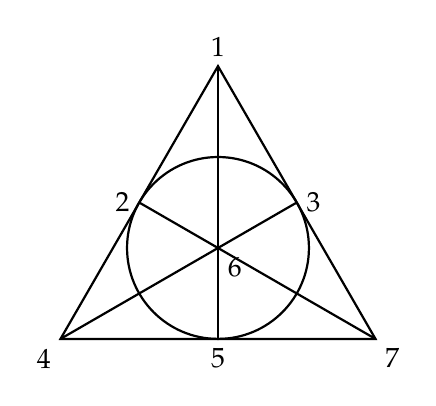
\begin{tikzpicture}[scale=1]
      %► Define the main triangle vertices
      \coordinate (A) at (2,3.464);   % point 1: apex
      \coordinate (B) at (0,0);       % point 4: left base
      \coordinate (C) at (4,0);       % point 7: right base
    
      %► Incenter and incircle radius
      \coordinate (O) at (2,1.155);   % point 6
      \def\radius{1.155}
    
      %► Touch‐points (midpoints)
      \coordinate (P) at ($(B)!0.5!(A)$);  % point 2
      \coordinate (Q) at ($(C)!0.5!(A)$);  % point 3
      \coordinate (R) at ($(B)!0.5!(C)$);  % point 5
    
      %► Draw everything
      \draw[line width=0.8pt] (A) -- (B) -- (C) -- cycle;      % triangle
      \draw[line width=0.8pt] (O) circle (\radius);          % incircle
      \draw[line width=0.8pt] (O) -- (P) -- (C);              % radii & chord
      \draw[line width=0.8pt] (O) -- (Q) -- (B);              % radii & chord
      \draw[line width=0.8pt] (O) -- (R);                     % radius to base
      \draw[line width=0.8pt] (A) -- (R);                     % altitude
  
      %► Labels
      \node[above]       at (A) {1};
      \node[left]        at (P) {2};
      \node[right]       at (Q) {3};
      \node[below left]  at (B) {4};
      \node[below]       at (R) {5};
      \node[below right] at (O) {6};
      \node[below right] at (C) {7};
    \end{tikzpicture}
    \caption{The Fano plane as a triangle with its inscribed circle and connecting lines.}
    \label{fig:Fano-plane}
\end{figure}

\begin{definition}
    The \emph{incidence matrix} $A = [a_{ij}]$ of a block design is a $v \times b$ matrix in which the rows correspond 
    to the \emph{varieties} (points) $x_1, \cdots, x_v$ and the columns to the blocks $B_1, \cdots, B_b$ whose $i, j$th entry is defined by 
    $$a_{ij} = \begin{cases}
        1 \quad &\text{if } x_i \in B_j \\
        0 \quad &\text{o.w}
    \end{cases}$$
    An example of the use of incidence matrices can be found on page 24. 
\end{definition}

\begin{remark}
    For binary codes, the sphere-packing bound turns out to be reasonably good for cases where $n \geq 2d + 1$. 
    However, for $n < 2d$, the bound becomes very weak. 
\end{remark}

\section{Linear Codes}

\begin{definition}
    A \emph{linear code} over $\mathbb{F}_q$ is simply a subspace of $\mathbb{F}_q^n$ for some positive integer $n$.
\end{definition}

In particular, a binary code is linear if and only if the sum of any two codewords is also a codeword.

\begin{definition}
    The \emph{dimension} of a linear code $C$ is the dimension of the subspace $C$ as a vector space over $\mathbb{F}_q$. 
    We denote this dimension by $k$, $C$ is said to be an \emph{[n,k]-code} or an \emph{[n,k,d]-code}.
\end{definition}

\begin{remark}
    \begin{enumerate}[label = (\roman*)]
        \item A $q$-ary $[n,k,d]$ code is a $q$-ary $(n, q^k, d)$ code, but the converse isn't necessarily true.
        \item $0_v \in C$ for any linear code $C$
    \end{enumerate}
\end{remark}

\begin{theorem}\label{thm:linear-code-dist}
    Let $C$ be a linear code and $w(C)$ be the smallest of the weights of the non-zero codewords of $C$. then
    $$d(C) = w(C)$$
\end{theorem}

\subsection{Advantages of linear codes}
\begin{enumerate}[label = \roman*)]
    \item We can find the minimum distance by examining only $M-1$ non-zero codewords. 
    \item We can specify a linear $[n,k]$-code by simply giving a basis of $k$ codewords.
    \item Linear codes are easy to encode and decode.
\end{enumerate}

\begin{definition}
    A $k \times n$ matrix whose rows form a basis of a linear $[n,k]$ code is called a \emph{generator matrix} of the code.
    This allows us to easily specify any linear code. 
\end{definition}

\subsection{Disadvantages of linear codes}

\begin{enumerate}[label = \roman*)]
    \item We can only define linear $q$-ary codes for $q$ power of a prime (Although we can construct some reasonnable $q$-ary codes over a larger alphabet). 
    \item The restriction to linear codes might restrict us to weaker codes than desired. 
\end{enumerate}

\subsection{Equivalence of linear codes}

\begin{definition}
    We say that two \textbf{\emph{linear codes}} are \emph{equivalent} if one can be obtained from the other by a combination of 
    \begin{itemize}
        \item permutation of the positions of the code 
        \item multiplication of the symbols in a fixed position by a non-zero scalar. 
    \end{itemize}
\end{definition}

\begin{theorem}
    Two $k \times n$ matrices generate equivalent linear $[n,k]$ codes over $\mathbb{F}_q$ iff one matrix 
    can be obtained from the other by a sequence of these operation: 
    \begin{itemize}
        \item[R1. ] Permutation of the rows 
        \item[R2. ] Multiplication of the row by a non-zero scalar 
        \item[R3. ] Addition of a scalar multiple of one row to another 
        \item[C1. ] Permutation of the columns 
        \item[C2. ] Multiplication of the columns by a non-zero scalar    
    \end{itemize}
    i.e the equivalence of linear codes is defined by the equivalence of their generator matrices.
\end{theorem}

\begin{theorem}
    Let $G$ be a generator matrix of an $[n,k]$-code, then it is a standard result from linear algebra that by performing elementary row and column operations we can 
    transform $G$ into the \emph{standard form} 
    $$ [I_k \mid A]$$
\end{theorem}

\section{Encoding and Decoding with linear codes} 

\subsection{Encoding with a linear code}

Given a linear code $C$ with generator matrix $G$, we can encode a message $u \in \mathbb{F}_q^k$ by computing the codeword
$$v = uG \in C$$
If $G$ is in standard form then simply 
$$x = uG = x_1 x_2 \cdots x_k x_{k+1} \cdot x_n$$
Where $x_1 \cdots x_k = u_1 \cdots u_k$ and 
$$x_{k+i} = \sum_{j=1}^{k} a_{ji}u_j \quad 1 \leq i \leq n - k$$
which are the \emph{check digits}, they represent the redundancy which has been added to the message to protect against noise. 

\subsection{Decoding with a linear code}

\begin{definition}
    Suppose the codeword $x = x_1 \cdots x_n$ is being sent through the channel and that the received 
    vector is $y = y_1 \cdots y_n$. We define the \emph{error} vector $e$ to be 
    $$e = y - x = e_1 \cdots e_n$$
\end{definition}

A decoder must decide from $y$ which codeword $x$ was transmitted, or equivalently which error $e$ has occured. 
An elegant nearest neoghbour decoding scheme uses the fact that a linear code is a subgroup of the additive subgroup of $\mathbb{F}_q^n$. 

\begin{definition}
    Th vector having minimum weight in a coset is called the \emph{coset leader}
\end{definition}

\begin{corollary}
    For any $C$ we can partition $\mathbb{F}_q^n$ into disjoint cosets of $C$: 
    $$\mathbb{F}_q^n = (0 + C) \cup (a_1 + C) \cup \cdots \cup (a_{q^{n-k} - 1} + C)$$
    where $a_1, \cdots, a_{q^{n-k} - 1}$ are taken to be the coset leaders.
\end{corollary}

\begin{definition}
    A (Slepian) \emph{standard array} for an $[n,k]$-code $C$ is a $q^{n-k} \times q^k$ array of all the vectors in 
    $\mathbb{F}_q^n$ in which the first row consists of the code $C$ with $0$ on the extreme left, and the other rows are the costs $a_i + C$, arranged in the same wayL with the coset leaders on the left. 
    There are standard algorithms which allow us to easily construct standard arrays.
\end{definition}

\begin{example}
    A standard array is of the form 
    \center
    \begin{array}{cccc}
        0000 & 1011 & 0101 & 1110 \\
        1000 & 0011 & 1101 & 0110 \\
        0100 & 1111 & 0001 & 1010 \\
        0010 & 1001 & 0111 & 1100
    \end{array}
\end{example}

When $y$ is received (e.g $1111$ in the example above), we find its position in the array, 
then the decoder decides that the vector $e$ is the coset leader ($0100$ in this example). Hence, 
it is decoded as the codeword $x = y - e (1011)$ at the top of teh column containing $y$. 

The errors vectors will always be the coset leaders, therefore by choosing a minimum weight vector as coset leader, 
we ensure that this is a nearest neighbor decoding scheme. 

\paragraph{Notes.}
This decoding shceme is too slow and costly (in terms of space) to be useful for larger codes. A more practical way to carry out this 
decoding is known as 'Syndrome decoding'. 

\subsection{Probability of error correction} 

\paragraph{Note. } We will restrict ourselves to binary codes. We will also assume 
that we are working in a bsc with error probability $p < 1/2$.

\begin{theorem}
    Let $C$ be a binary $[n,k]$-code, and for $i = 0 \cdots n$, let $\alpha_i$ be the numbers 
    of coset leaders of weight $i$. Then 
    $$P_{\text{corr}}(C) = \sum_{i = 0}^{n} \alpha_i p^i (1 - p)^{n-i}$$
    and thus the \emph{word error rate} is 
    $$P_{\text{error}}(C) = 1 - P_{\text{corr}}(C)$$
\end{theorem}

\begin{definition}
    The \emph{rate} of a code $C$ is defined as the ratio of the number of information symbols to the total number of symbols in the codeword, i.e: 
    $$R(C) = \frac{k}{n}$$
    where $k$ is the dimension of the code and $n$ is the length of the codeword.
\end{definition}

\begin{definition}
    The \emph{capacity} $\mathscr{C}(p)$ of a $\operatorname*{bsc}(p)$ is 
    $$\mathscr{C}(p) = 1 + p \log_2 p + (1-p) \log_2 (1-p)$$
\end{definition}

\begin{theorem}\label{thm:Shannon-thms}
    Suppose that we have a $\text{bsc}(p)$, Let $R < \mathscr{C}(p)$
    therefore for any $\varepsilon > 0$, there exists $n \in \mathbb{N}$ s.t we have an 
    $[n,k]$-code $C$ of rate of rate $R$ with 
    $$P_{\text{err}}(C) < \varepsilon$$

    Similarly, if $R > \mathscr{C}(p)$, then no sequence of $[n,k]$ codes with rate 
    $$R > \mathscr{C}(p)$$
    can have vanishing error probability. 
\end{theorem}

In plainer terms: 
\begin{itemize}
    \item if $R < \mathscr{C}$ then we can make $P_{\text{err}} \to 0$. 
    \item if $R > \mathscr{C}$ then we can't make $P_{\text{err}} \to 0$.
\end{itemize}

\subsection{Probability of error detection} 

Notice that if we use our binary linear code only for error detection, we make an error if and only if $e$ is a (nonzero) valid codeword. 
Therefore $P_{\text{undetec}}(C)$ is indepedendent of the codeword sent. 

\begin{theorem}
    Let $C$ be a binary $[n,k]$-code and let $A_i$ denote the number of codewords of $C$ of weight $i$. Then 
    $$P_{\text{undetec}}(C) = \sum_{i = 1}^{n} A_i p^i (1-p)^{n-i}$$
\end{theorem}

\section{Dual codes, Parity check matrices, and Syndrome decoding}

\subsection{Dual codes} 

\begin{definition}
    Given a linear $[n,k]$-code $C$, the \emph{dual code} of $C$, denoted by $C^\perp$, is defined as such 
    $$C^\perp = \{v \in \mathbb{F}_q^n \mid \| v \cdot u = 0 \quad \forall u \in C\}$$
    It is a standard fact from linear algebra that $C^\perp$ is a 
    linear $[n, n-k]$-code. 
\end{definition}

\begin{proposition}
    \begin{itemize}
        \item If $C_1$ and $C_2$ are equivalent linear codes, then so are 
        $C_1^\perp$ and $C_2^\perp$. 
        \item $(C^\perp)^\perp = C$. 
    \end{itemize}
\end{proposition}

\subsection{Parity check matrices} 

\begin{definition}
    A \emph{parity-check matrix} $H$ for an $[n,k]$-code $C$ is a generator matrix of $C^\perp$.

    Thus, $H$ is an $(n-k) \times n$ matrix such that
    $$GH^T = 0$$
\end{definition}

\begin{theorem}
    Let $H$ be a parity check matrix for $C$, then 
    $$C = \{x \in \mathbb{F}_q^n \mid \| xH^T = 0\}$$
    Hence, any linear code is entirely determined by its parity check matrix. 
\end{theorem}

The rows of a parity check matrix are \emph{parity checks} on the codewords; they say that certain 
linear combination of the coordinates of every codeword are zero. 

\begin{example}
    if 
    $$H = \begin{pmatrix}
        1 & 1 & 0 & 0 \\
        0 & 0 & 1 & 1
    \end{pmatrix}$$
    then $C$ is the code 
    $$C = \{(x_1, x_2, x_3, x_4) \in \mathbb{F_2}^4 \mid \| x_1 + x_2 = 0, \, x_3 + x_4 = 0\}$$
\end{example}

\begin{theorem}\label{thm:standard-form-parity-check}
    If $G = [I_k \mid A]$ is the standard from generator matrix of an $[n,k]$-code $C$, then a parity check matrix for $C$ is 
    $H = [-A^T|I_{n - k}]$.  
\end{theorem}

\begin{definition}
    By analogy, we say that a parity check matrix is in \emph{standard form} iff
    $$H = [-A^T | I_{n-k}]$$
\end{definition}

\subsection{Syndrome decoding}

\begin{definition}
    Let $H$ be a parity check matrix of an $[n,k]$-code $C$. Then for any 
    vector $y \in \mathbb{F}_n^q$, we define the \emph{syndrome} of $y$ to be the $1 \times (n - k)$ row vector
    $$S(y) = y H^T$$ 
    (Some people define the syndrome as the column vector $S(y) = H y^T$ instead, but this is equivalent).
\end{definition}

\begin{proposition}
    \begin{itemize}
        \item if the rows of $H$ are $h_1, \cdot, h_{n-k}$, then 
        $$S(y) = (y \cdot h_1, y \cdot h_2, \cdots, y \cdot h_k)$$
        \item $$S(y) = 0 \iff y \in C$$
    \end{itemize}
\end{proposition}

\begin{proposition}
    There is a one-to-one correspondence between syndromes and cosets (Since $u, v \in \mathbb{F}_q^n$ are in the same coset iff they have the the same syndrome). 
\end{proposition}

Notice that this allows to replace the standard array decoding (in a more efficient manner). 
We can use the syndrome to find out which coset (row of the array)
contains $y$. We do this as follows: 
\begin{enumerate}[label = \roman*)]
    \item Calculate the syndrome $S(e)$ for each coset leader $e$. 
    \item When $y$ is received, calculate $S(y) = y H^T$ and locate $S(y)$. 
    \item The coset leader $e$ corresponding to $S(y)$ is the error vector.
\end{enumerate}

\begin{example}
    Consider the code with generator matrix 
    $$G = \begin{pmatrix}
        1 & 0 & 1 & 1 \\
        0 & 1 & 0 & 1
    \end{pmatrix}$$
    Therefore by theorem \ref{thm:standard-form-parity-check}, a parity check matrix for this code is
    $$ H = \begin{pmatrix}
        1 & 0 & 1 & 0 \\
        1 & 1 & 0 & 1
    \end{pmatrix}$$
    Hence the syndromes of the cosets leaders are 
    \begin{align*}
        S(0000) &= 00 \\
        S(1000) &= 11 \\
        S(0100) &= 01 \\
        S(0010) &= 10
    \end{align*}
    Which gives us the syndrome lookup table: 
    \begin{table}[H]
        \centering
        \begin{tabular}{cc}
            \hline
            Syndrome $z$ & Coset leader $e$ \\
            \hline 
            $00$ & $0000$ \\
            $11$ & $1000$ \\
            $01$ & $0100$ \\
            $10$ & $0010$ 
        \end{tabular}
    \end{table}
    Which allows us to find $e$ efficiently. 
\end{example}

\subsection{Incomplete decoding} 

This is a blend of error correction and detection. More precisely, if $d(C) = 2t + 1$ or $d(C) = 2t + 2$; 
then we guarantee the correction of $\leq t$ errors in any codeword and also detect some cases of more than $t$ errors. 

We sort the cosets in order of increasing weights, and divide the array into a 
\emph{top part} comprising of the cosets whose leaders have weights $\leq t$, and a \emph{bottom part} comprising those remaining cosets. 
If the received vector $y$ is in the top part, we decode it as usual; if $y$ is in the bottom part, we conclude that more than $t$ error have occured and ask for retransmission. 

\begin{example}
    Let $C$ be the binary code with generator 
    $$ \begin{pmatrix}
        1 & 0 & 1 & 1 & 0 \\
        0 & 1 & 0 & 1 & 1
    \end{pmatrix}$$
    A standard array for $C$ is 
    \center
    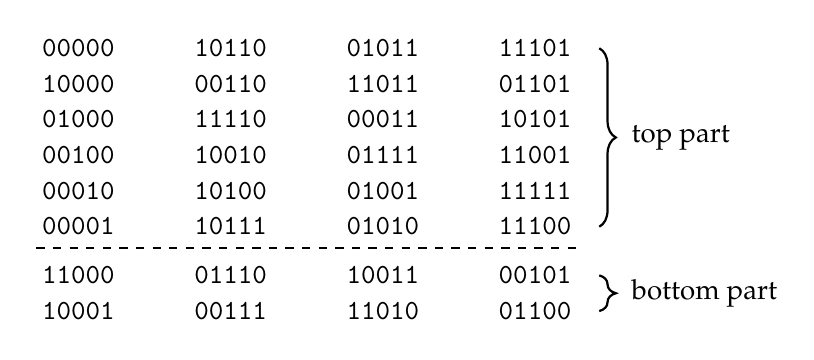
\begin{tikzpicture}
        % Styles
        \tikzset{
          bit/.style={
            font=\ttfamily,
            inner sep=0pt,
            minimum width=3em,
            text height=1.5ex, text depth=0.25ex
          },
          partbrace/.style={
            decorate,
            decoration={brace,amplitude=6pt},
            thick
          }
        }
      
        % 8×4 matrix of bit‐strings
        \matrix (m) [
          matrix of nodes,
          nodes=bit,
          column sep=2.5em,
          row sep=1ex
        ]{
          00000 & 10110 & 01011 & 11101 \\
          10000 & 00110 & 11011 & 01101 \\
          01000 & 11110 & 00011 & 10101 \\
          00100 & 10010 & 01111 & 11001 \\
          00010 & 10100 & 01001 & 11111 \\
          00001 & 10111 & 01010 & 11100 \\[1ex] % extra gap
          11000 & 01110 & 10011 & 00101 \\
          10001 & 00111 & 11010 & 01100 \\
        };
      
        % dashed separator just below row 6
        \draw[dashed, thick]
          ($(m-6-1.south west)+(0,-0.7ex)$) --
          ($(m-6-4.south east)+(0,-0.7ex)$);
      
        % top‐part brace (shifted right by 0.8em)
        \draw[partbrace]
          ($(m-1-4.east)+(0.8em,0)$) --
          ($(m-6-4.east)+(0.8em,0)$)
          node[midway, right=8pt] {top part};
      
        % bottom‐part brace
        \draw[partbrace]
          ($(m-7-4.east)+(0.8em,0)$) --
          ($(m-8-4.east)+(0.8em,0)$)
          node[midway, right=8pt] {bottom part};
    \end{tikzpicture}
    If $11110$ is received, we decode it as $10110$, but if $10011$ is received, we seek re-transmission. 
\end{example}

The point here is that in the lower part, nearest neighbor decoding ends in a tie, therefore probability of decoding is low. 
An incomplete scheme is particularly useful for codes with even minimum distance. Since if $d(C) = 2t + 2$, then we can guarantee correction of up to $t$ errors
and simultaneously detect up to $t + 1$ errors.

Another advantage of incomplete decoding is that we don't need to use the full standard array (even in the construction). This 
is because we know that the coset leaders of the top part are precisely the vectors of weight $\leq t$.

\section{The Hamming codes} 

Hamming codes are linear codes which are easy to encode and decode, they can be defined over any $\mathbb{F}_q$ but we will restrict ourselves 
to the binary case. 

\begin{definition}
    Let $r$ be a positive integer and let $H$ be an $r \times (2^r - 1)$ matrix whose columns are the distinct non-zero vectors of 
    $\mathbb{F}_r^2$. Then the \emph{Hamming code} $\text{Ham}(r,2)$ is the code having $H$ as its parity check matrix.

    We will generalize this later to $\text{Ham}(r, q)$ for any prime power $q$.
\end{definition}

\paragraph{Notes.} 
\begin{itemize}
    \item $\text{Ham}(r,2)$ has length $n = 2^r - 1$ and dimension $k = n - r$. 
    Thus, $r = n - k$ is the number of check symbols and is known as the \emph{redundancy} of the code. 
    \item The order in the columns of $H$ don't matter, hence $\text{Ham}(r, 2)$ is for given $r$ any of the equivalent codes. 
\end{itemize}

\begin{theorem}\label{thm:hamming-code-properties}
    The binary Hamming code $\text{Ham}(r,2)$ for $r \geq 2$ : 
    \begin{enumerate}[label = (\roman*)]
        \item is a $[2^r - 1, 2^r - 1 - r]$-code ($M = 2^{2^r - 1 - r}$).
        \item has minimum distance $d = 3$. 
        \item is  a perfect code. 
    \end{enumerate}    
\end{theorem}

\subsection{Decoding the binary Hamming code} 

Since $\text{Ham}(r, 2)$ is a perfect single error correcting code, the coset leaders 
are precisely the $2^r (= n + 1)$ vectors of weight $\leq 1$. 

The syndrome of a received vector $e_j^T$ is simply 
\begin{align*}
    e_j^T H^T &= (H e_j)^T \\
    &= h_j^T 
\end{align*}
Where $h_j$ denotes the $j$'th column of $j$. 

Hence, by arranging the columns of $H$ in increasing order, we get a nice decoding algorithm. 
\begin{enumerate}
    \item Calculate the syndrome $S(y) = y H^T$.
    \item If $S(y) = 0$, then $y$ is a codeword (assume no error). 
    \item if $S(y) \neq 0$, (assume single error) then $S(y)$ gives the binary 
    representation of the error position. 
\end{enumerate}

\subsection{Extended binary Hamming codes} 

\begin{definition}
    The \emph{extended binary Hamming code} $\text{Ham}^e(r, 2)$ is the code obtained from $\text{Ham}(r, 2)$ 
    by adding an extra parity check symbol to each codeword. 
\end{definition}

\begin{proposition}
    By theorem \ref{thm:parity-check-codes}, we get that 
    $$\text{Ham}^e(r,2) \text{ is a } [2^r, 2^r-1-r, 4] \text{ code}$$ 
\end{proposition}

\paragraph{Note.} The extended code $\text{Ham}^e(r,2)$ is no better than $\text{Ham}(r,2)$ when used for complete decoding. 
In fact, it is inferior since an extra check digit is required per codeword (lower rate). However, it is suited for incomplete decoding since 
it can correct any single error and detect any double error. 

\paragraph{Construction.} Let $H$ be a parity-check matrix for $\text{Ham}(r,2)$. A parity matrix $\tilde{H}$ for the extended 
code is 
$$\tilde{H} = \begin{pmatrix}
    & & & & 0 \\
    & & & & 0 \\
    & & H & & \cdots \\
    & & & & 0 \\
    1 & 1 & \cdots & 1 & 1 
\end{pmatrix}$$
The last row gives us the overall parity check 
$$x_1 + x_2 + \cdots + x_{n+1} = 0$$

\paragraph{Decoding.} By taking $H$ in increasing order of binary numbers, there is a neat 
decoding algorithm. 
\begin{enumerate}[label = (\roman*)]
    \item if both parity check bit and syndrome are $0$, assume no errors. 
    \item if parity check is zero but syndrome is non-zero, seek retransmission. 
    \item if parity check is one but syndrome is zero, assume error in the parity check. 
    \item if parity check and syndrome are non-zero, decode as usual.
\end{enumerate}

\subsection{q-ary Hamming codes}

\begin{theorem}\label{thm:distance-to-parity-check}
    Suppose $C$ is a linear $[n,k]$-code over $\mathbb{F}_q$ with parity-check matrix $H$. Then the minimum distance of $C$ is $d$ 
    if and only if any $d - 1$ columns of $H$ are L.I but some $d$ columns are linearly dependent.
\end{theorem}

Notice that this result is twofold: 
\begin{enumerate}
    \item It establishes the minimum distance of a specific linear code when $H$ is given
    \item It allows us to construct a parity-check matrix to provide a code of guaranteed minimum distance. 
\end{enumerate}

We will be focusing here on the case where $d = 3$. I.e we require that any two columns of $H$ to be 
L.I (no zero vector, and no scalar multiples). 

Any non-zero $v \in \mathbb{F}_q^r$ has exactly $q-1$ non-zero scalar multiples. Thus the $q^r - 1$ non-zero vectors
of $\mathbb{F}_q^r$ may be partitionned into $(q^r - 1) / (q-1)$ such classes. 

By choosing one vector from each class, we obtain a set of $(q^r - 1) / (q-1)$ 
vectors, which are pairwise L.I. 

Hence, by theorem \ref{thm:distance-to-parity-check}, taking these as the columns of $H$ gives a parity-check matrix
for a linear $[(q^r - 1)/(q-1), (q^r - 1)/(q-1) - r, 3]$-code. 

\begin{definition}
    The linear code constructed above is called \emph{$q$-ary Hamming code} 
    and is denoted $\text{Ham}(r,q)$.  
\end{definition}

\paragraph{Note.} Different parity-check matrices may be chosen to define $\text{Ham}(r,q)$ 
for given $r$ and $q$, all of these matrices are equivalent. Therefore the Hamming codes are linear codes 
which are uniquely defined, up to equivalence, for their parameters. 

An easy way to write down a parity-check matrix for $\text{Ham}(r, q)$ is to list as columns all non-zero $r$-tuples 
of $\mathbb{F}_q^r$ with first-nonzero entry equal to $1$. 

\begin{theorem}\label{thm:Hamming-perfect}
    $\text{Ham}(r,q)$ is a perfect single-error-correcting code. 
\end{theorem}

\begin{corollary}
    If $q$ is a prime power and $n = \frac{q^r - 1}{q - 1}$ for some $r \geq 2$, 
    then 
    $$A_q(n, 3) = q^{n-r}$$
\end{corollary}

\paragraph{Decoding with a $q$-ary  Hamming code}

Since a Hamming code is a perfect single-error correcting code, the coset leaders, other than 
$0$ are precisely the vectors of weight $1$.  The syndrome of such a coset leader is 
$$S(b \cdot e_j^T) = b H_j^T$$

Therefore we can decode as folllows: 
\begin{enumerate}[label = \roman*)]
    \item Calculate $S(y) = y H^T$. 
    \item if $S(y) = 0$, assume no errors. 
    \item if $S(y) \neq 0$, then $S(y) = b H_j^T$ for some $b$ and $j$, therefore we correct the 
    assumed errr by substracting $b$ from the $j$'th entry of $y$. 
\end{enumerate}

\subsection{Shortening a code}

Shortening a code is useful if we want a code of given length and distance and we know a good code of 
greater length and same minimum distance. 

\begin{definition}
    Let $C$ be a $q$-ary $(n,M,d)$ code. Consider a fixed coordinate position $j$ and a fixed symbol 
    $\lambda$ of the alphabet. 
    Then, if we take all the codewords of $C$ having $\lambda$ in the $j$th position and delete the $j$th coordinate from these codewords, 
    we will get $C'$ a code of length $n-1$, in general, fewer codewords but the same minimum distance. 
    $C'$ is called an \emph{shortened} code of $C$. 
\end{definition}

\paragraph{Note.} If $C$ is a linear $[n,k,d]$-code and the deleted symbol is a $0$, then $C'$ will also be linear: 
it will ba a $[n-1,k-1,d']$-code where $d' \geq d$ (in general $d' = d$). 
Moreover, if $C$ has parity-check matrix $H$, then it is easy to see that a paritiy check matrix of $C'$ is obtained by deleting the corresponding 
column of $H$. 

\subsection{The Gilbert-Varshamov bound} 

\begin{theorem}\label{thm:GV-bound}
    Let $q$ be a primer power, then there exists a $q$-ary $[n,k]$-code with minimum 
    distance at least $d$ provided that 
    $$\sum_{i = 0}^{d -2} (q-1)^i \binom{n-1}{i} < q^{n-k}$$
\end{theorem}

\begin{corollary}
    If $q$ is a prime-power then 
    $$A_q(n,d) \geq q^k_1$$
    Where $k_1$ is the largest integer $k$ such that 
    $$q^k < \frac{q^n}{\sum_{i = 0}^{d-2} (q-1)^i \binom{n-1}{i}}$$
\end{corollary} 

\section{Other good codes} 


\begin{definition}
A family of linear codes $\{\,C_n\}_{n=1}^\infty$, where each $C_n$ is an $[n,k_n,d_n]$ code over a fixed finite field, is called \emph{good} if there exist constants $R>0$ and $\delta>0$ such that for all sufficiently large $n$:
\[
\frac{k_n}{n} \;\ge\; R,
\qquad
\frac{d_n}{n} \;\ge\; \delta,
\]
and with a poly-time decoding algortihm. 
\end{definition}

\subsection{Hadamard Code and Generalization} 

\paragraph{Hadamard Matrices}
\begin{definition}
    A square matrix $H$ of order $n$ with elements $+1$ and $-1$ such that 
    $H H^T = n I_n$ is called a \emph{Hadamard matrix} 
\end{definition}

We will demonstrate a way to construct Hadamard matrices: 

\begin{definition}
    If $A$ is an $m \times m$ matrix with entries $a_{ij}$ and $B$ is an $n \times n$ matrix, then the Kronecker product 
    $A \otimes B$ is the $mn \times mn$ matrix given by 
    $$A \otimes B := \begin{pmatrix}
        a_{11}B & a_{12}B & \cdots & a_{1m}B \\
        a_{21}B & a_{22} B & \cdots & a_{2m} B \\
        \vdots & \vdots & \ddots & \vdots \\
        a_{m1} B & a_{m2} B & \cdots & a_{mm} B 
    \end{pmatrix}$$
\end{definition}

It can be shown that the Kronecker product of Hadamard Matrices is a Hadamard matrix. 
Starting from $H_2 := \begin{pmatrix}
    1 & 1 \\
    1 & -1 
\end{pmatrix}$ we can find the sequence $H_2^{\otimes n}$, where $H_2^{\otimes 2} = H_2 \otimes H_2$, etc. 

Note that this only allows us to construct a small subset of the Hadamard matrices (the Sylvester matrices), there exist other construction schemes.

\paragraph{Hadamard Codes} 
\begin{definition}
    The \emph{Hadamard code} of order $n$ is the linear code obtained in general by the construction below:
    
    Let $H_n$ be a Hadamard matrix of order $n$. In $H_n$ and $- H_n$ we replace $-1$ by $0$. 
    This allows us to find $2n$ rows which are in $\mathbb{F}_2^n$. Since any two rows of a Hadamard matrix differ in half of the positions, 
    we have constructed a $(n, 2n, 1/2 n)$ code (For $n = 8$, this is an extended Hamming code). 
\end{definition}

\subsection{Low-Density Parity-Check Codes} 
\begin{definition}
    A \emph{low-density parity-check code} (or Gallager code) is a block code that has a parity check matrix $H$, 
    every row and column of which is sparse. 

    A \emph{regular} LDPC is a code in which every column of $H$ has the same weight $j$ and every row has the same 
    weight $k$. 
\end{definition}

For any column weight $j \geq 3$, LDPC codes are \emph{good codes}. Moreover, some sequences of 
LDPC codes have the ratio $j / N \to 0$.  

However, we don't have an optimal decoder, and decoding these codes is an NP-complete problem. In practice,
these codes are decoded using \emph{iterative message-passing}, which works well against random errors. 
\section{Reference}
All material is adapted from: 
\begin{quote}
    \textbf{Raymond Hill}, \emph{A First Course in Coding Theory}, Oxford University Press, 1986.
    \textbf{J.H. van Lint}, \emph{Introduction to Coding Theory}, Springer, 3rd Edition, 1999.
\end{quote}
Page or chapter references will are given in the text where relevant. 
\end{document}
